
\chapter{Payload}
\label{chap:payload}

Without a Payload there is no mission. It gives meaning and purpose to the system. The payload itself is very important for the design and layout of a rover system. The components of the payload carried along are examined in detail below. 

\section{Ground RADAR}
The Ground Radars main task is the identification of suitable drilling sites. Additionally every radar campaign will contribute to further understanding of the ground composition on Europa.

due to its small dimensions the CRUX GPR is selected . The system is tested for lunar application at 800~MHz resulting in a resolution of 15~cm and a penetration depth of 5~m \cite{CRUX_GPR}. The INSPIRE mission makes use of a 1.5~GHz frequency to increase the resolution. 
Reduced penetration depths are acceptable since the depth of interest for the ice core sampling is 10~cm.

Additionally high frequencies lead to compact antenna design which is beneficial to the INSPIRE mission due to weight constraints. 
A custom patch antenna with the properties in \autoref{tab:GPR-A-Prp} is proposed \cite{patch_ant_GPR}\cite{Patch_Ant_design}. \autoref{fig:DrillBay}

\begin{table}[h]
\centering
\begin{tabular}{lllll}
\toprule
Substrate ${\varepsilon}_\text{r}$ & Width & Length & Height & Mass   \\
\midrule
20                         & 30 mm & 20 mm  & 2 mm   & 2,73 g  \\
\bottomrule
\end{tabular}
\caption{GPR antenna properties \cite{Patch_Ant_design}}
\label{tab:GPR-A-Prp}
\end{table}

\section{Ice Core Drill}

The ice core drill is an in-house development which is based on the NanoDrill from Honeycomp and the drill from Philae. The drill bit is made out of titanium to ensure that it does not deform or even break through during the drilling process.
The ice core sample that can be obtained has a length of 100~mm and a diameter of 10~mm
In order to save space, the drill is folded in while driving and will unfold for drilling, which is illustrated in the following \autoref{fig:DrillBay}.
When the drilling process is finished, it is folded in again and the trap doors are closed.
Now the sample can be pushed out with the help of a plunger and meanwhile it can be analyzed by the APXS sensor. 
When the sample has left the drill body and the analysis is completed, the rover can switch back to Locomotion mode and look for a new place to drill. As soon as a new drilling process will started, the previously taken sample falls to the ground to make room for a new one.


\begin{figure}[htb]
     \centering
     \begin{subfigure}[b]{0.49\textwidth}
         \centering
         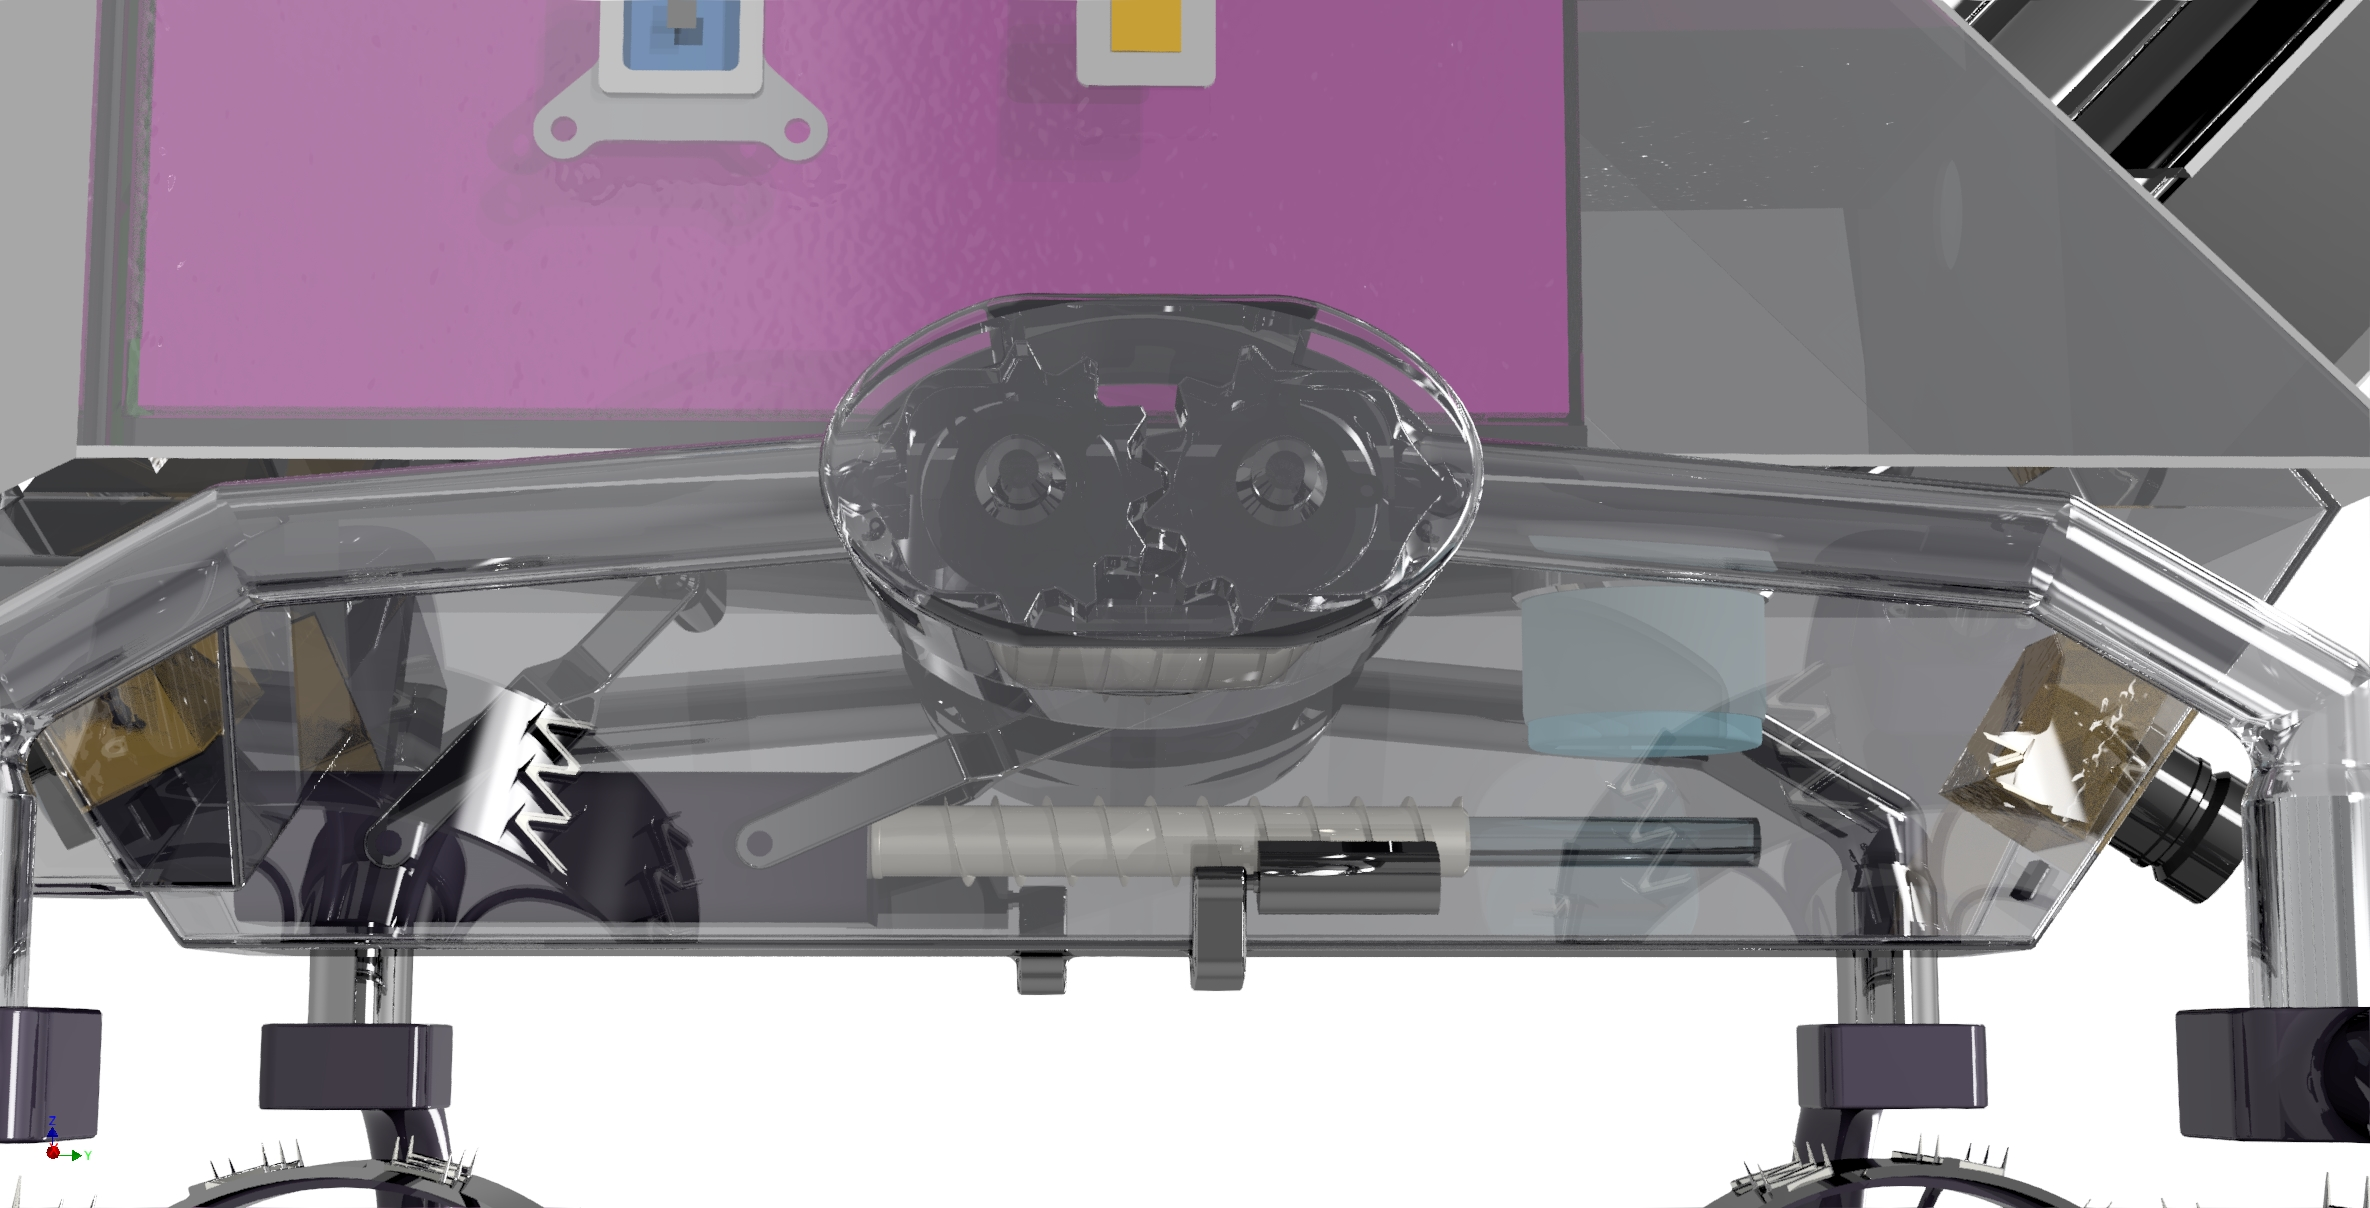
\includegraphics[width=\textwidth]{Media/DrillingBay3}
         \label{fig:stowedDrill}
     \end{subfigure}
     \hfill
     \begin{subfigure}[b]{0.49\textwidth}
         \centering
         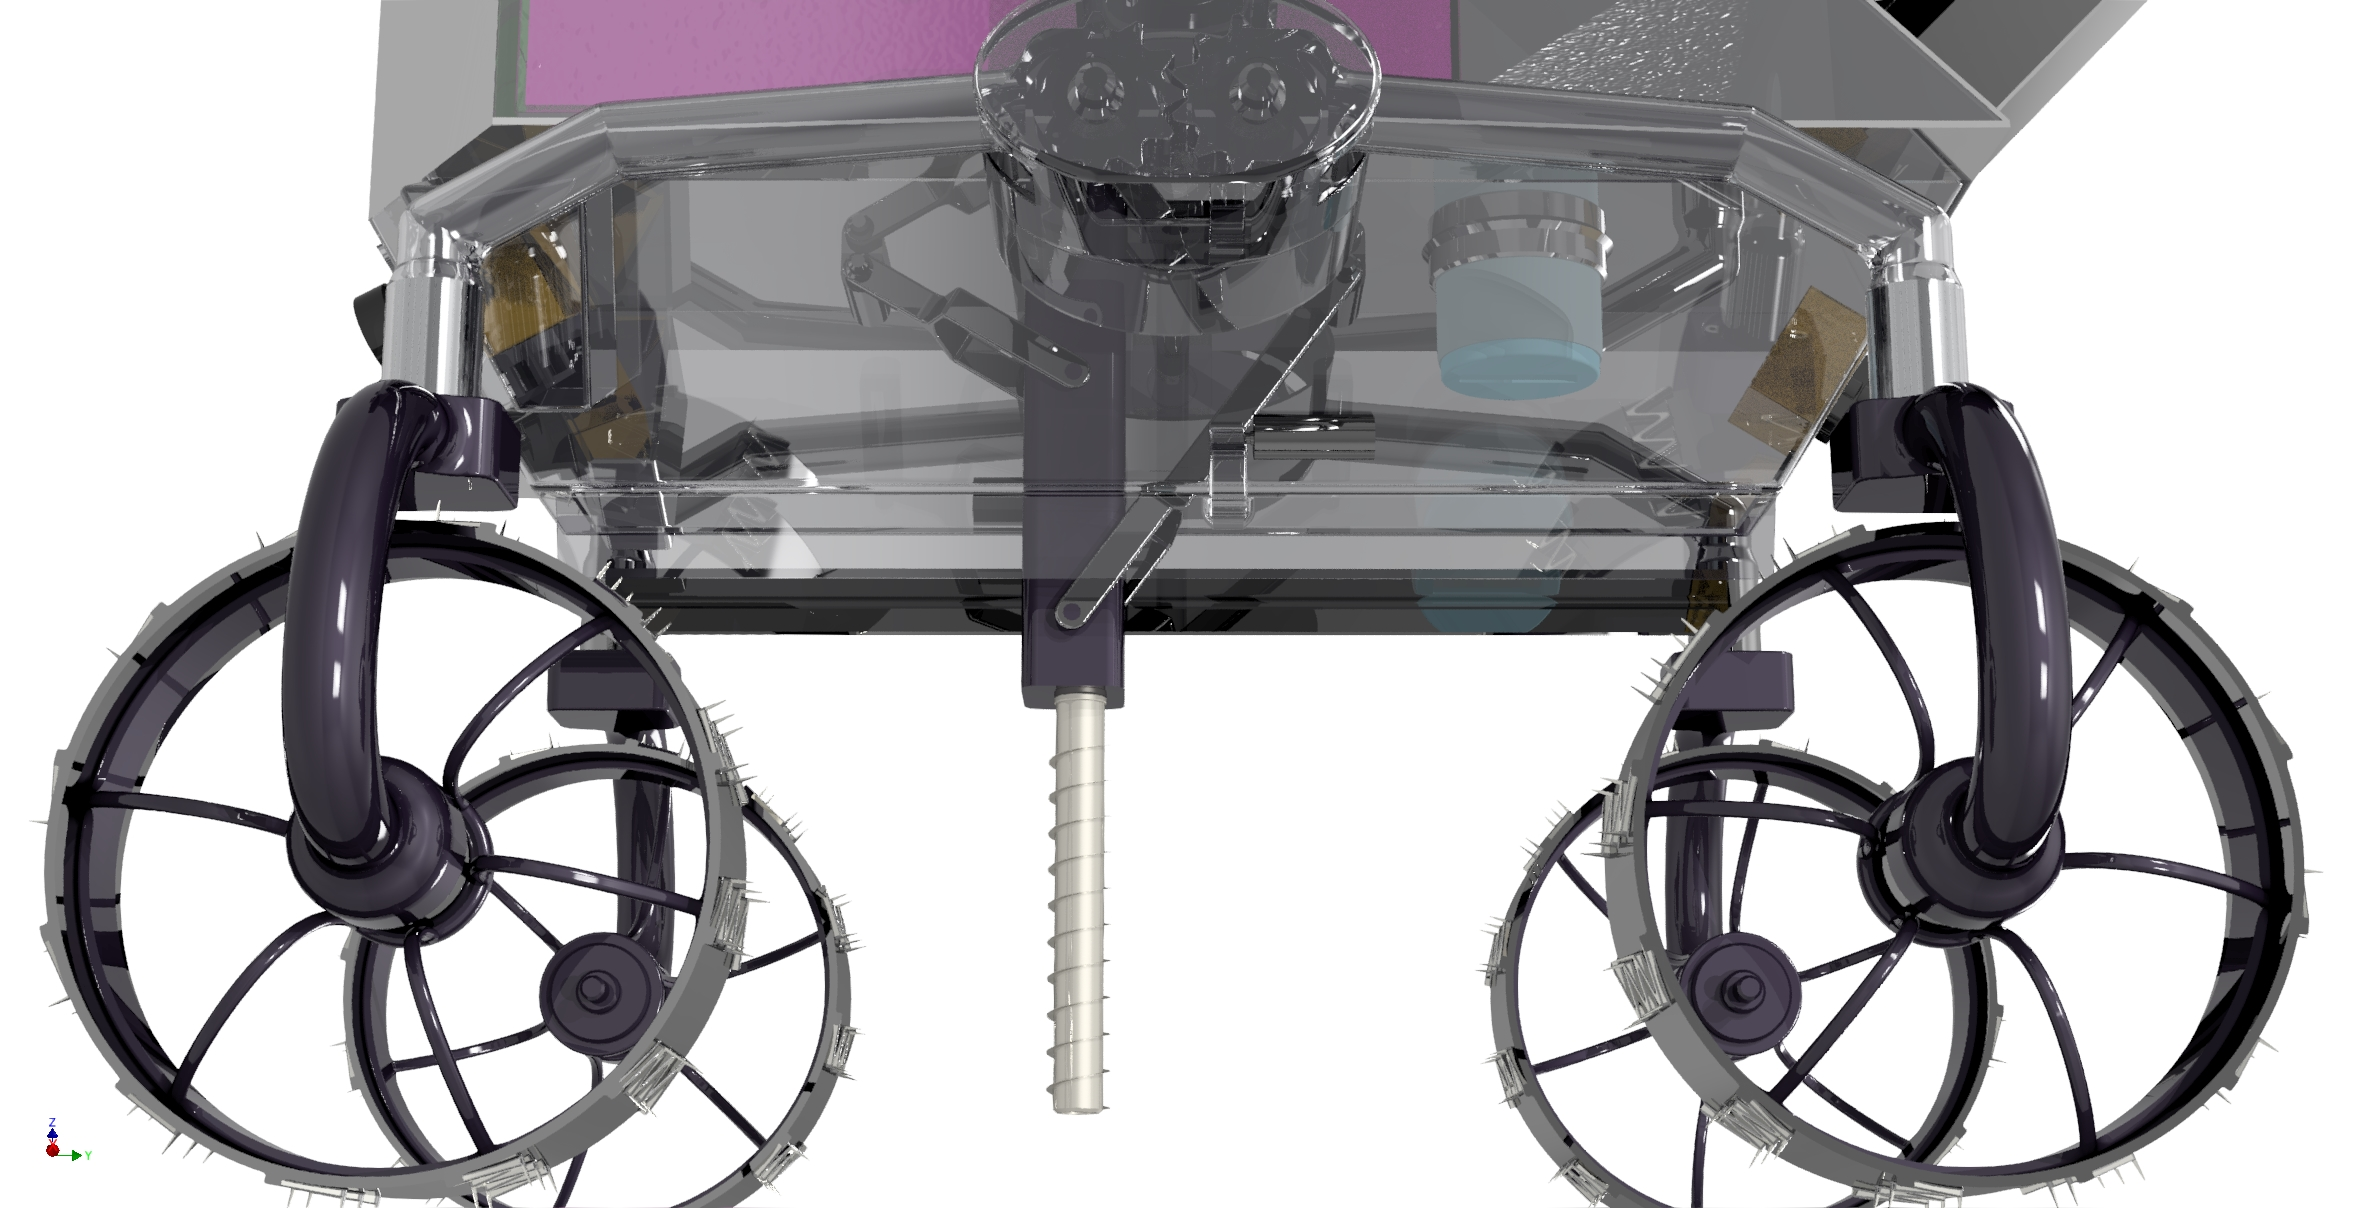
\includegraphics[width=\textwidth]{Media/DrillingBay_unfolded2}
         \label{fig:drillconfig}
     \end{subfigure}
     \hfill
     \caption{Left: Ice Core Drill in stowed configuration inside the chassi, Right: Ice Core Drill in drilling configuration}
     \label{fig:DrillBay}
\end{figure}

\section{APXS Analyzer}
The Alpha Particle X-Ray Spectrometer is an analyser which has been used in many explorer missinons like the philae lander or the mars rover Curiosity, \cite{ref_pay_1} \cite{ref_pay_2}.
The spectrometer uses alpha particles as well as X-ray to identify the sort of atom inside a probe.
The main advantage is the small mass and the  low power it needs during the operation.
As a result of the  quite thin ice core samples actual one third of APXS sources and detectors will used.
Therefore the mass and the power consumtion was down sized by one third because the electronic keeps the same and can't be reduced.


\section{Stereovision Camera / Observation / Perception}

The INSPIRE rover is equipped with five individual cameras. Two are used as stereo vision cameras on an hight adjustable and rotatable telescope arm on the front side of the rover. This is used to capture a detailed 3D model of the environment with which sizes and distances can be estimated. The remaining three cameras are used as haz-cameras which are necessary to obtain data regarding the nearby environment. All cameras are equipped with radiation hardened lenses to prevent browning of the lenses. Additional information is provided in \autoref{app:DigitalAppendix}. The main tasks of the camera system is the provision of scientific data and navigation related data. %More details regarding the navigation and autonomy are provided in \autoref{sec:ControlandAutonomy}. \autoref{fig:CamHEad}

\begin{figure}[htb]
     \centering
     \begin{subfigure}[b]{0.49\textwidth}
         \centering
         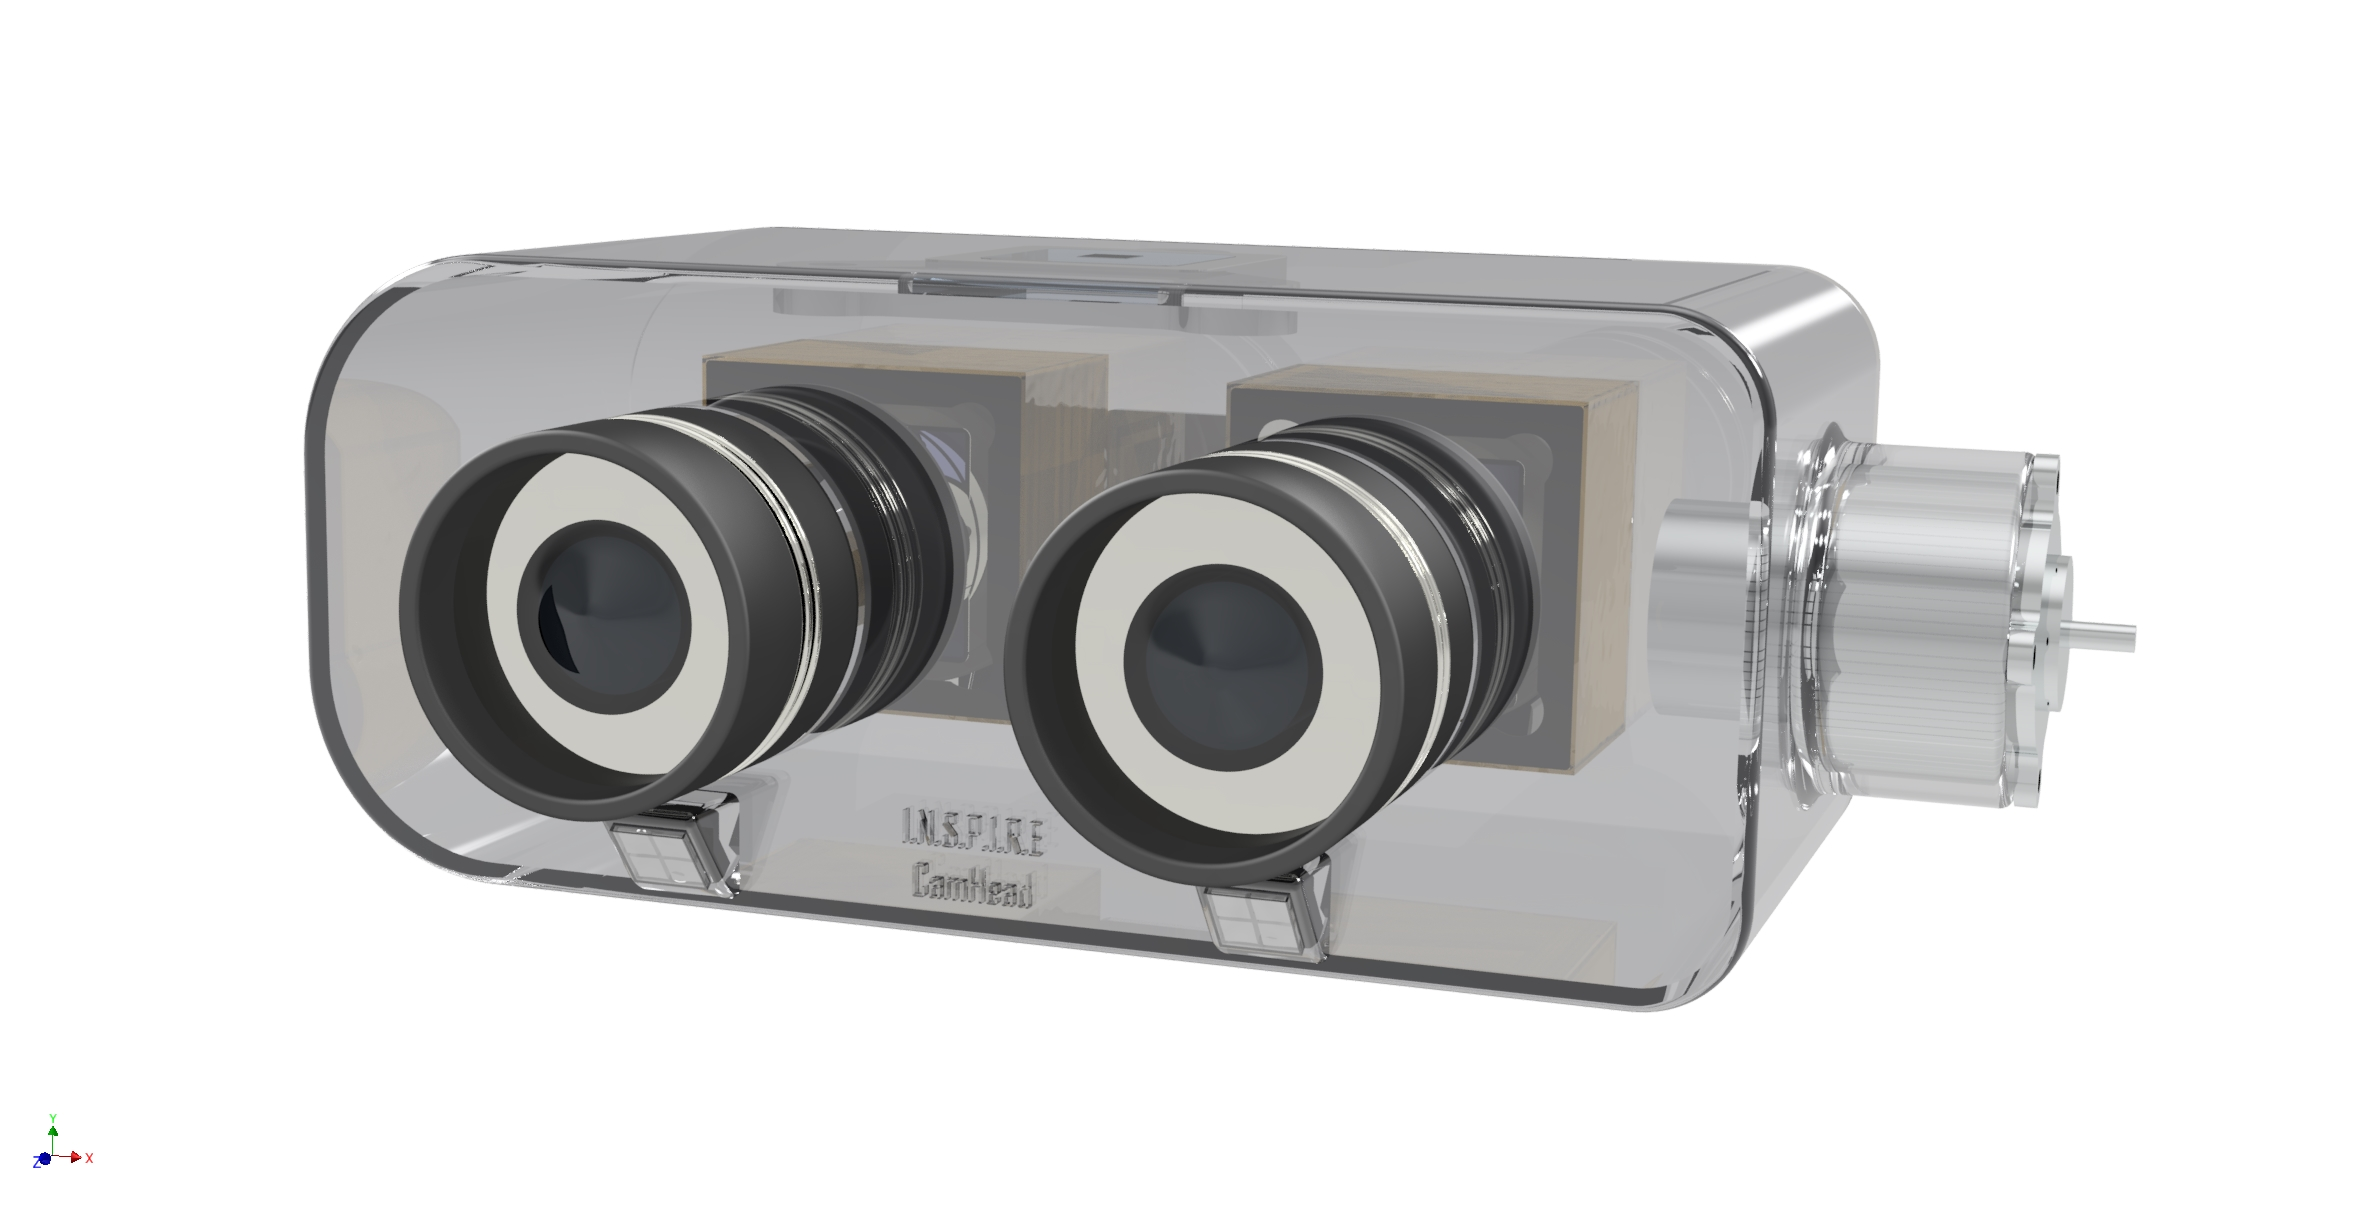
\includegraphics[width=\textwidth]{Media/CamHead}
         \label{fig:CamHead}
     \end{subfigure}
     \hfill
     \begin{subfigure}[b]{0.49\textwidth}
         \centering
         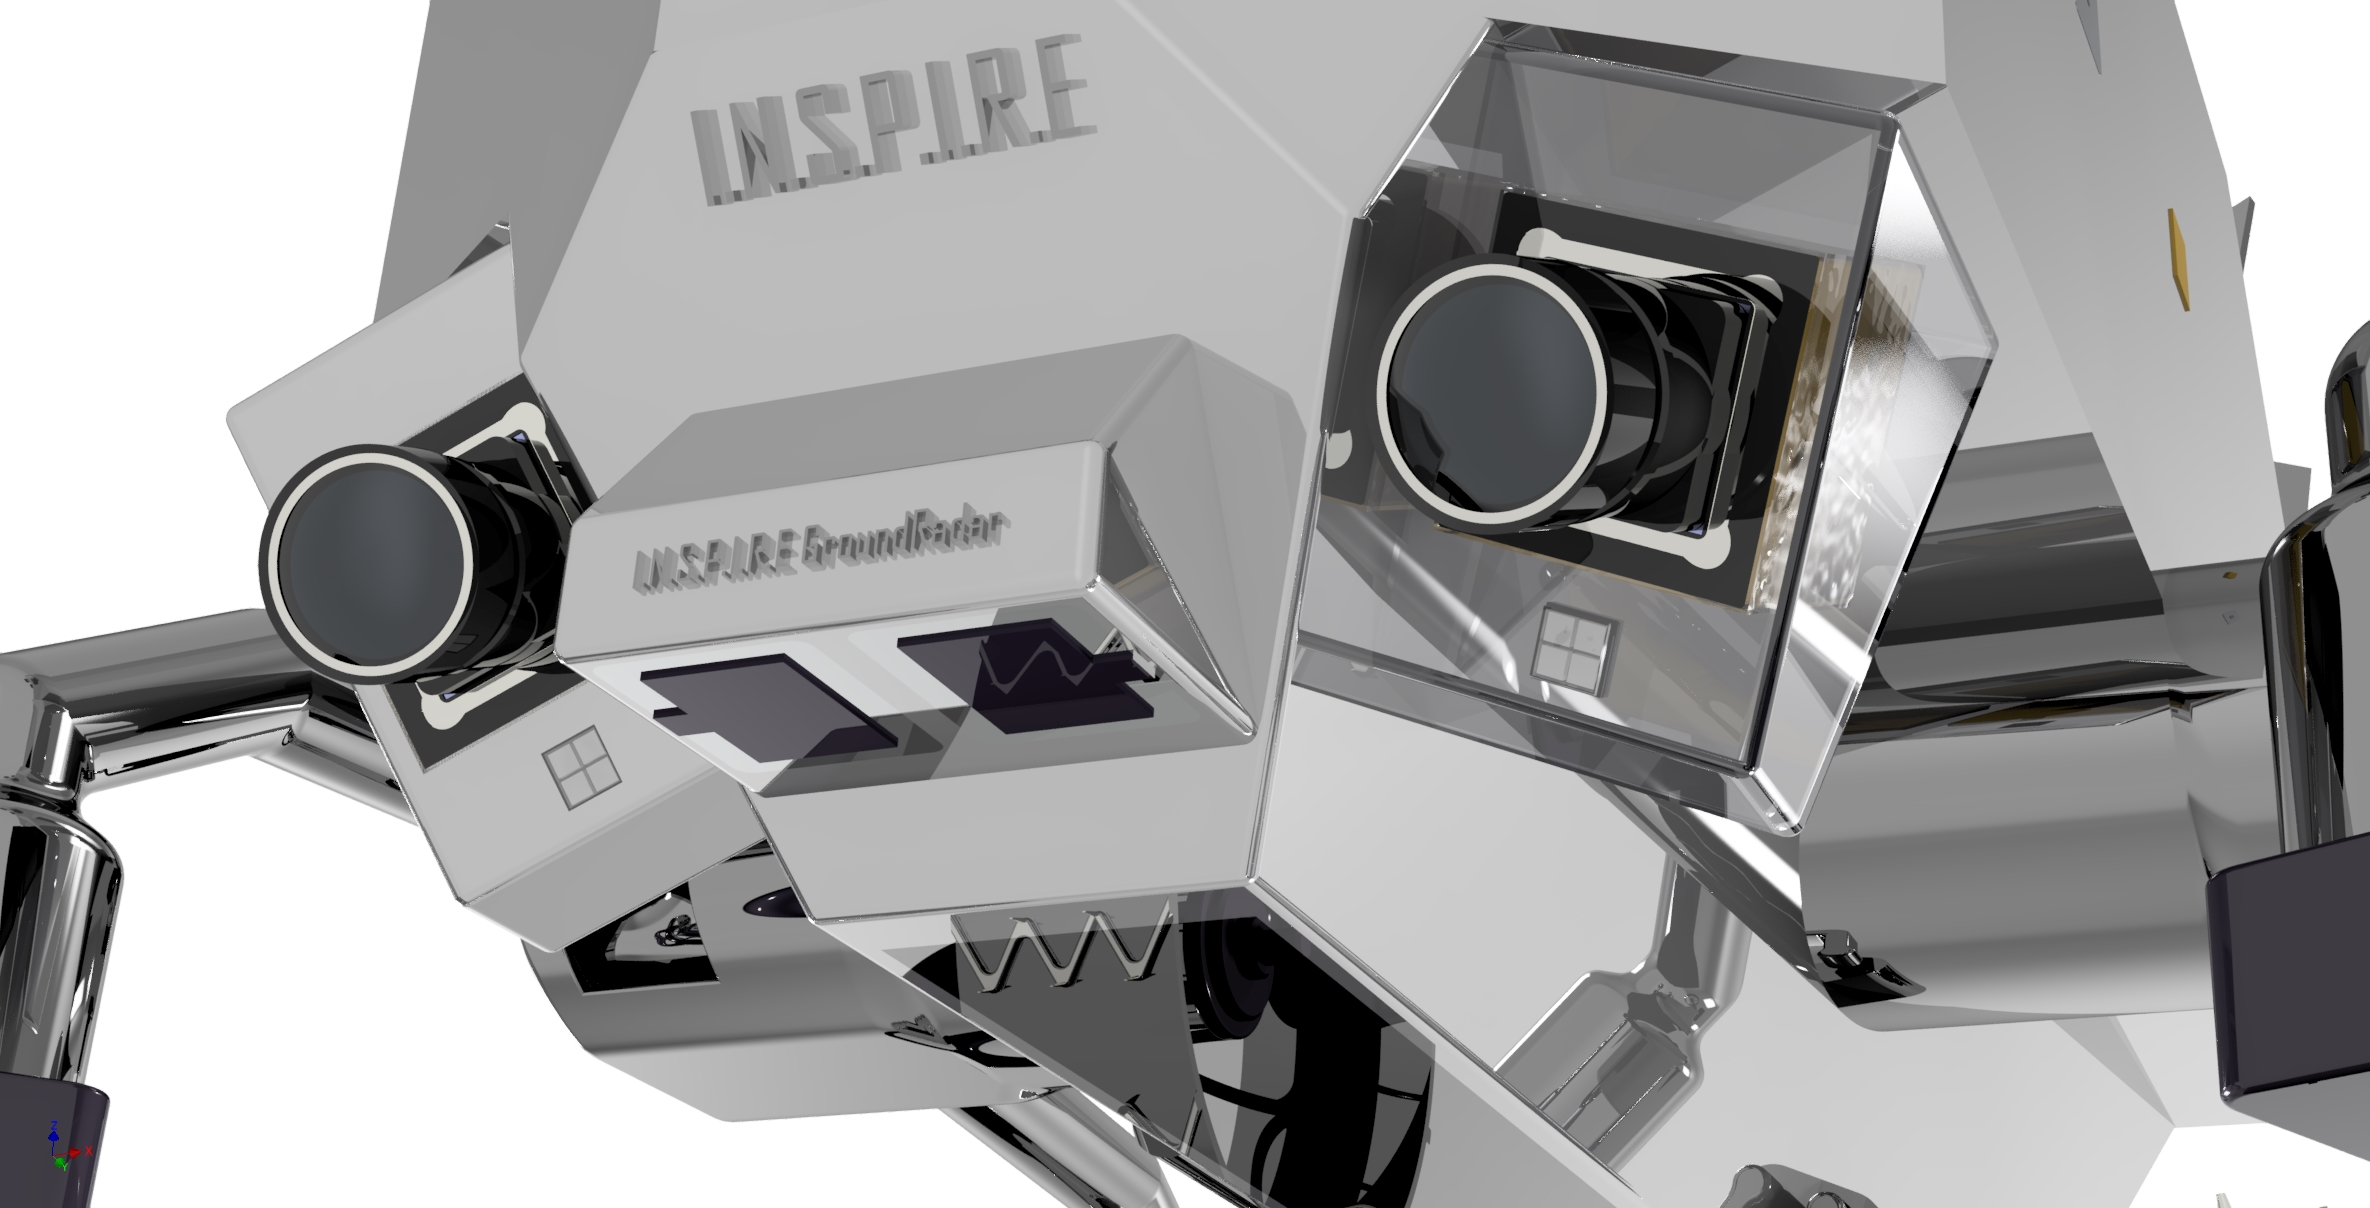
\includegraphics[width=\textwidth]{Media/HazCam_GroundRadar}
         \label{fig:HazCam}
     \end{subfigure}
     \hfill
     \caption{INSPIRE's Surface Observation System including CamHead and Haz Cams + Ground Radar}
     \label{fig:Observation}
\end{figure}

\section{RadHard Solar Arrays}
\label{subsec:radhard}
As a secondary mission goal for INSPIRE a cooperation with the european project RadHard which is led by the german solar array manufacturer Azure Space is intended. They are currently developing a new generation of $4$ Junction solar cells with an efficiency of up to $35~\% $. But the main feature of the new solar arrays is their radiation hardness which will be the highest radiation hardness ever designed with an efficiency of $>3~\% $ after $1E15~\text{cm}^{-2} \ 1~\text{MeV}$ electron irradiation. So the Jupiter environment with its extreme radiation would be the best suitable destination for a test and evaulation mission of this new technology. Therefore INSPIRE will be equipped with $10$ RadHard solar cells with a total surface area of $0.0310~\text{m}^2$ for a technology demonstration \cite{FraunhoferInstituteforSolarEnergySystemsISE.2021}.

